\section{実験結果と考察\label{result}}

\subsection{RQ1 : レコードはOSSにおいて,どの程度の数使用されているのか?\label{rq1_result}}

\begin{figure}[t]
    \centering
    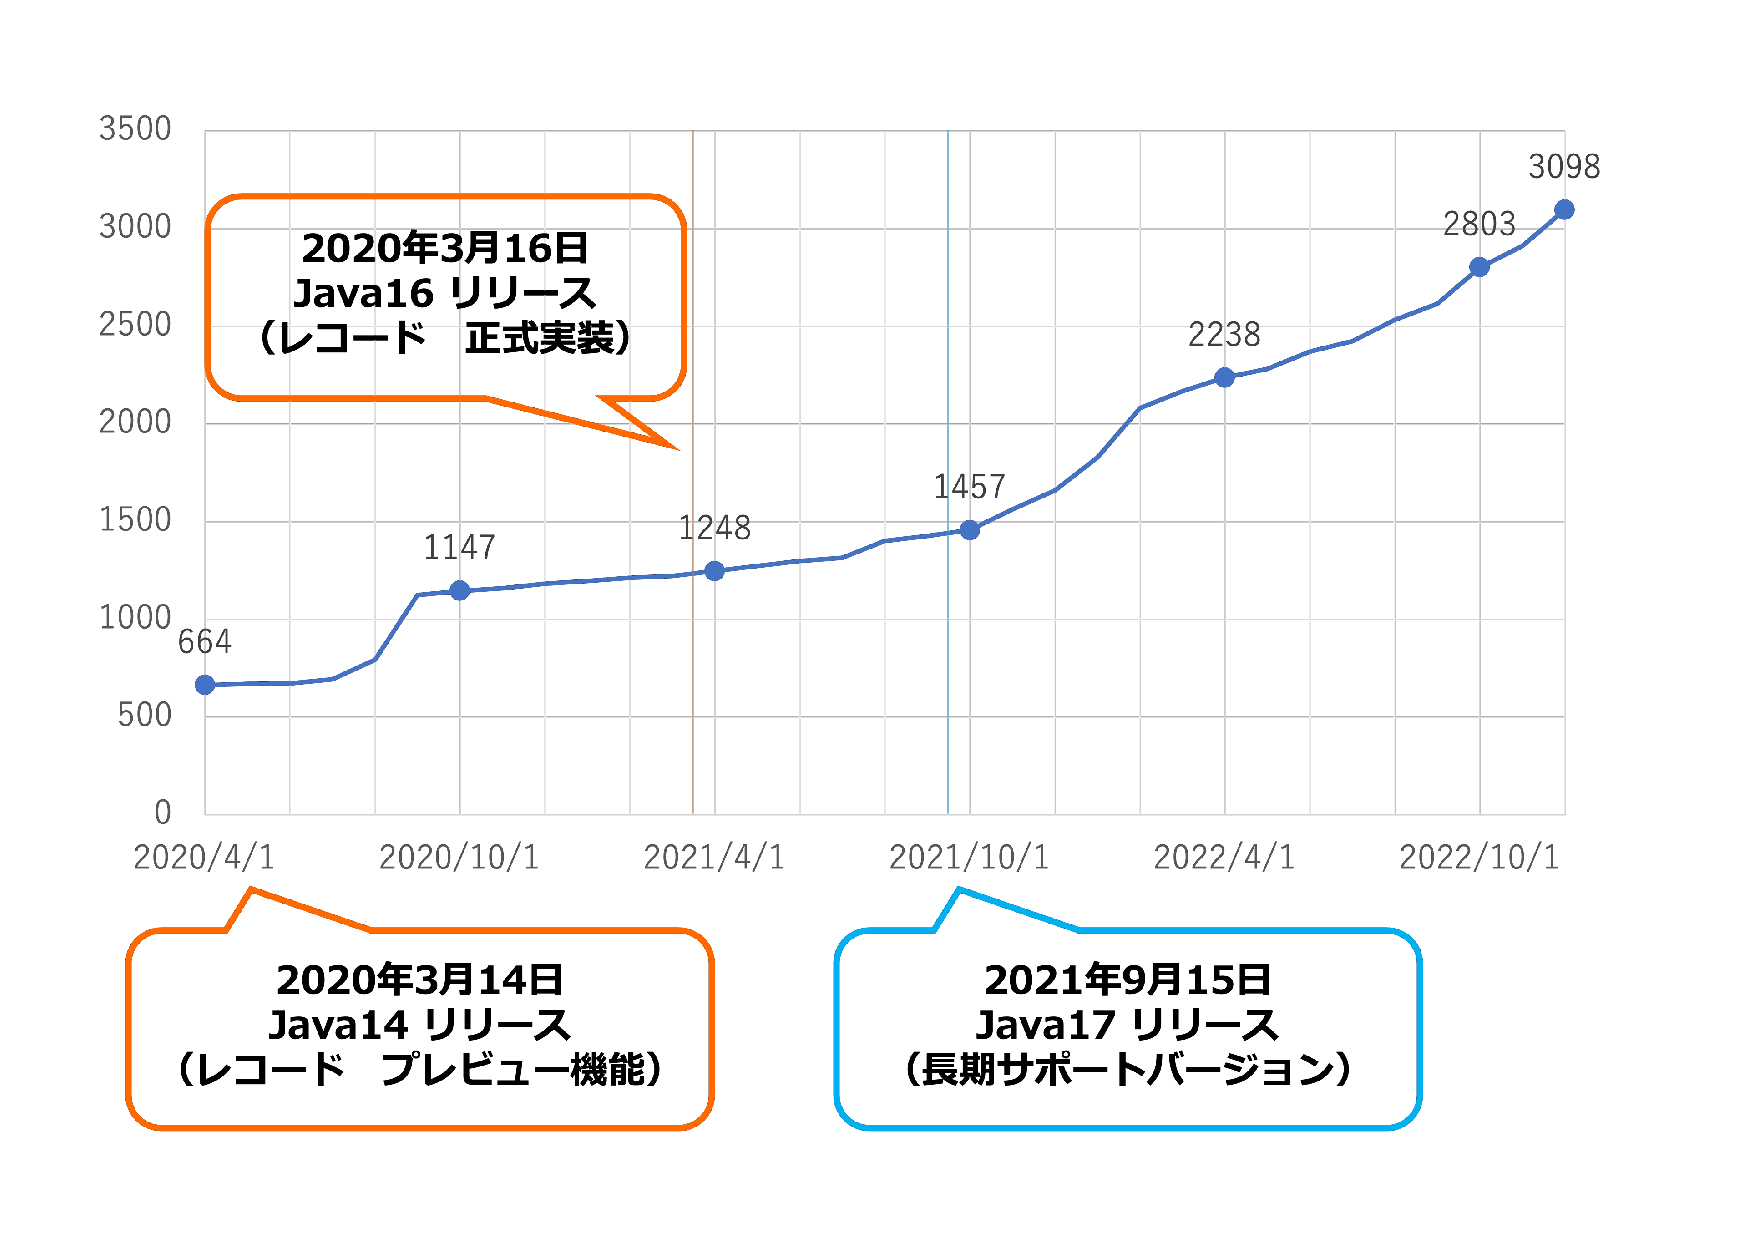
\includegraphics[width=10cm]{image/num_records.pdf}
    \caption{レコードの利用数の変遷}
    \label{num_records}
\end{figure}

\figref{num_records}は,2020年4月から2022年12月までのレコード利用数の変遷を示した折れ線グラフである.
データセットのレポジトリをクローンした2022年12月25日時点では,70件のレポジトリで合計3,244件のレコードが利用されていた.
利用数の伸び方に注目してみると,Java17がリリースされる2020年9月までの18か月の区間は月44.1件のペース,2020年10月以降の14か月の区間は月117.2件のペースでレコードが導入されている.
すなわち,レコードの利用数の伸びはJava17の登場以降に加速していることがわかる.

\subsection{RQ2 : 使用されているレコードの特徴はどのようになっているか?\label{rq2_result}}
\subsubsection{インスタンスフィールド数\label{num_instance_fields}}

\begin{table}[t]
    \caption{定義フィールド個数別のレコード(クラス)の件数}
    \label{num_fields}
    \centering
    \begin{tabular}{c||r|r|r|r}
        \hline
        フィールド数 & \multicolumn{2}{c|}{レコード} & \multicolumn{2}{c}{クラス}\\
         & 個数 & 割合 & 個数 & 割合\\
        \hline\hline
        0 & 317 & 9.8\% & 229,275 & 60.9\%\\
        1 & 815 & 25.1\% & 54,129 & 14.4\%\\
        2 & 1,070 & 33.0\% & 32,501 & 8.6\%\\
        3 & 483 & 14.9\% & 19,358 & 5.1\%\\
        4 & 205 & 6.3\% & 12,043 & 3.2\%\\
        5 & 129 & 4.0\% & 8,115 & 2.2\%\\
        6\textasciitilde10 & 157 & 4.8\% & 15,174 & 4.0\%\\
        11\textasciitilde & 68 & 2.1\% & 6,077 & 1.6\%\\
        \hline
        合計 & 3,244 & - & 376,672 & - \\
        \hline
    \end{tabular}
\end{table}

\tabref{num_fields}は,レコードおよびクラスのインスタンスフィールド数別に,件数を集計したものである.
最も多かったのはフィールド数が2個のレコードで,全体の33.0\%を占めていた.
なお,定義1件あたりのフィールド数を算出したとことろ,クラスは1.85個であるのに対し,レコードは2.88個であった.
すなわち,レコードの方がクラスよりも多くのフィールドを持つことがわかった.

\subsubsection{フィールド型の傾向\label{field_type_trend}}

\begin{table}[t]
    \caption{レコードのフィールド型の傾向}
    \label{record_field_types}
    \centering
    \begin{tabular}{c||r|r}
        \hline
        型名 & 個数 & 割合\\
        \hline\hline
        int & 2,871 & 30.7\%\\
        (java.lang.)String & 1,725 & 18.4\%\\
        long & 615 & 6.6\%\\
        boolean & 374 & 4.0\%\\
        double & 205 & 2.2\%\\
        List<String> & 109 & 1.2\%\\
        (java.lang.)Boolean & 74 & 0.8\%\\
        double[] & 68 & 0.7\%\\
        (java.lang.)Object & 65 & 0.7\%\\
        (java.lang.)Integer & 64 & 0.7\%\\
        その他 & 3,182 & 34.0\%\\
        \hline
        合計 & 9,352 & -\\
        \hline
    \end{tabular}
\end{table}

\begin{table}[t]
    \caption{クラスのフィールド型の傾向}
    \label{class_field_types}
    \centering
    \begin{tabular}{c||r|r}
        \hline
        型名 & 個数 & 割合\\
        \hline\hline
        long & 205,434 & 29.4\%\\
        int & 77,043 & 11.0\%\\
        (java.lang.)String & 53,182 & 7.6\%\\
        boolean & 39,275 & 5.6\%\\
        (java.lang.)Object & 5,829 & 0.8\%\\
        double & 4,408 & 0.6\%\\
        byte[] & 3,875 & 0.6\%\\
        List<String> & 3,501 & 0.5\%\\
        int[] & 3,398 & 0.5\%\\
        float & 3,246 & 0.5\%\\
        その他 & 298,946 & 42.8\%\\
        \hline
        合計 & 698,137 & - \\
        \hline
    \end{tabular}
\end{table}

% \begin{table}[t]
%     \caption{レコード(クラス)のフィールド型の傾向}
%     \label{field_types}
%     \centering
%     \begin{tabular}{c||r|r||c||r|r}
%         \hline
%         型名 & \multicolumn{2}{c||}{レコード} & 型名 &\multicolumn{2}{c|}{クラス}\\
%          & 個数 & 割合 & & 個数 & 割合\\
%         \hline\hline
%         int & 2,871 & 30.7\% & long & 205,434 & 29.4\%\\
%         (java.lang.)String & 1,725 & 18.4\% & int & 77,043 & 11.0\%\\
%         long & 615 & 6.6\% & (java.lang.)String & 53,182 & 7.6\%\\
%         boolean & 374 & 4.0\% & boolean & 39,275 & 5.6\%\\
%         double & 205 & 2.2\% & (java.lang.)Object & 5,829 & 0.8\%\\
%         List<String> & 109 & 1.2\% & double & 4,408 & 0.6\%\\
%         (java.lang.)Boolean & 74 & 0.8\% & byte[] & 3,875 & 0.6\%\\
%         double[] & 68 & 0.7\% & List<String> & 3,501 & 0.5\%\\
%         (java.lang.)Object & 65 & 0.7\% & int[] & 3,398 & 0.5\%\\
%         (java.lang.)Integer & 64 & 0.7\% & float & 3,246 & 0.5\%\\
%         その他 & 3,182 & 34.0\% & その他 & 298,946 & 42.8\%\\
%         \hline
%         合計 & 9,352 & - & 合計 & 698,137 & - \\
%         \hline
%     \end{tabular}
% \end{table}

% \begin{table}[t]
%     \caption{レコード(クラス)のフィールド型の傾向(種類別)}
%     \label{field_type_attributes}
%     \centering
%     \begin{tabular}{c||r|r|r|r}
%         \hline
%         型の種類 & \multicolumn{2}{c|}{レコード} & \multicolumn{2}{c}{クラス}\\
%          & 個数 & 割合 & 個数 & 割合\\
%         \hline\hline
%         プリミティブ型計 & 4,199 & 44.9\% & 333,636 & 47.8\%\\
%         プリミティブ配列型計 & 160 & 1.7\% & 14,400 & 2.1\%\\
%         ラッパークラス型計 & 224 & 2.4\% & 6,653 & 1.0\%\\
%         セット型計 & 95 & 1.0\% & 4,861 & 0.7\%\\
%         リスト型計 & 339 & 3.6\% & 19,217 & 2.8\%\\
%         マップ型計 & 158 & 1.7\% & 11,824 & 1.7\%\\
%         \hline
%     \end{tabular}
% \end{table}

\tabref{record_field_types}はレコードのインスタンスフィールド型,\tabref{class_field_types}はクラスのインスタンスフィールド型の傾向を集計したものである.
型の中にはjava.lang.Stringのように完全限定名で指定されているものもあったので,それらも単純名での検出と一緒にして計上している.
結果をみると,レコードのフィールド型として際立って利用されているのはint型であり,全体の30.7\%を占めている.
対してクラスのフィールド型として際立っているのはlong型であり,全体の29.4\%を占めている.
ただしこの数値は,レポジトリSapMachineとJetBrainsRuntimeにおける,大量のlong型フィールドを含むクラス群を計上した結果である.
これらのレポジトリには,わずか2つで合計81,903ものlong型フィールド宣言(全long型フィールドの39.9\%)を行うクラスが含まれており,結果に大きな影響を与えている.

SapMachineとJetBrainsRuntimeを除いた場合,レコードのフィールド型で最も多いのはStringで1,410件(全体の22.6\%),次点はintで1,177件(全体の18.9\%)となる.
一方,クラスのフィールド型で最も多いのはintで41,969件(全体の13.1\%),次点はStringで35,687件(全体の11.2\%)となる.

% そして\tabref{field_types_attributes}は,フィールド型を分類して集計したものである.
% Javaコレクションフレームワークの分類\cite{Collections_Framework}を参考にし,セット型はSet,HashSet,TreeSet,LinkedHashSetの4つ,リスト型はList,ArrayList,LinkedListの3つ,マップ型はMap,HashMap,TreeMap,LinkedHashMapの4つとしている.
% また,ジェネリクス及びrawタイプは区別していない.


\subsubsection{実装インタフェース数\label{num_implemented_interfaces}}

\begin{table}[t]
    \caption{実装インタフェース数別のレコード(クラス)の件数}
    \label{num_interfaces}
    \centering
    \begin{tabular}{c||r|r|r|r}
        \hline
        インタフェース数 & \multicolumn{2}{c|}{レコード} & \multicolumn{2}{c}{クラス}\\
         & 件数 & 割合 & 件数 & 割合\\
        \hline\hline
        0 & 2,443 & 75.3\% & 309,354 & 82.1\%\\
        1 & 743 & 22.9\% & 58,507 & 15.5\%\\
        2 & 54 & 1.7\% & 6,719 & 1.8\%\\
        3 & 4 & 0.1\% & 1,430 & 0.4\%\\\
        4\textasciitilde & 0 & 0.0\% & 662 & 0.2\%\\
        \hline
        合計 & 3,244 & - & 376,672 & - \\
        \hline
    \end{tabular}
\end{table}

\tabref{num_interfaces}は,レコードおよびクラスの実装インタフェース数別に,件数を集計したものである.
実装インタフェース数の平均をとると,レコードは0.266,クラスは0.213であるので,レコードの方がインタフェースの実装が行われやすいということがわかった.

\subsubsection{実装インタフェースの傾向\label{interface_trend}}

\begin{table}[t]
    \caption{レコードの実装インタフェースの傾向}
    \label{record_interface_types}
    \centering
    \begin{tabular}{c||r|r}
        \hline
        型名 & 件数 & 割合\\
        \hline\hline
        (java.io.)Serializable & 253 & 29.3\%\\
        Writeable & 49 & 5.7\%\\
        Decoration & 35 & 4.1\%\\
        Comparable & 34 & 3.9\%\\
        ToXContentObject & 30 & 3.5\%\\
        ThrowingExternalizable & 26 & 3.0\%\\
        ClusterStateTaskListener & 16 & 1.9\%\\
        ExpirationPolicyBuilder & 16 & 1.9\%\\
        ToXContentFragment & 15 & 1.7\%\\
        Runnable & 14 & 1.6\%\\
        その他 & 375 & 43.5\%\\
        \hline
        合計 & 863 & -\\
        \hline
    \end{tabular}
\end{table}

\begin{table}[t]
    \caption{クラスの実装インタフェースの傾向}
    \label{class_interface_types}
    \centering
    \begin{tabular}{c||r|r}
        \hline
        型名 & 個数 & 割合\\
        \hline\hline
        (java.io.)Serializable & 4,242 & 5.3\%\\
        Runnable & 3,225 & 4.0\%\\
        (java.util.)Iterator & 1,343 & 1.7\%\\
        (java.lang.)Comparable & 1,034 & 1.3\%\\
        (java.lang.)Cloneable & 888 & 1.1\%\\
        Collector & 811 & 1.0\%\\
        Writeable & 790 & 1.0\%\\
        ActionListener & 740 & 0.9\%\\
        ToXContentObject & 721 & 0.9\%\\
        IdentifiedDataSerializable & 606 & 0.8\%\\
        その他 & 65,649 & 82.0\%\\
        \hline
        合計 & 80,049 & -\\
        \hline
    \end{tabular}
\end{table}

\tabref{record_field_types}はレコードのインスタンスフィールド型,\tabref{class_field_types}はクラスのインスタンスフィールド型の傾向を集計したものである.
こちらも\ref{field_type_trend}節と同じく,完全限定名の指定と単純名の指定をまとめてある.また,型引数のある型は型引数を無視してまとめてある(rawタイプも含む).
結果を見ると,レコードもクラスも最も多く実装されているのは(java.io.)Serializableとなった.
ただ全体で見た比率に差があり,レコードは7.8\%,クラスは1.1\%への実装となっている.
クラスのみへの実装が際立っているインタフェースとしてはRunnableが挙げられる.
レコードにおいては全体の0.4\%程度だが,クラスでは全体の0.9\%となっている.

\subsection{RQ3 : クラスをレコードに変更するリファクタリングでは,どの程度の恩恵を享受できるのか?\label{rq3_result}}

\subsubsection{レコードの追加と削除の件数}
コミットで変更されたファイルの履歴からレコードの追加と削除を抽出し,分類を行った.
なお,ラムダ式などの内部で宣言されているレコードはクラスパスが生成できず,差分間で同一の型を特定するのが困難であるので,ここではトップレベルレコード及びクラス内部レコードのみを対象としている.
\tabref{record_addition}にレコードの追加の内訳,\tabref{record_addition}にレコードの削除の内訳を示す.

\begin{table}[t]
    \caption{レコードの追加の内訳}
    \label{record_addition}
    \centering
    \begin{tabular}{c||r|r}
        \hline
        型名 & 件数 & 割合\\
        \hline\hline
        新規ファイルと共に追加 & 2,096 & 67.0\%\\
        非レコード型からレコードへの変更 & 695 & 22.2\%\\
        既存ファイルへ追加 & 336 & 10.7\%\\
        \hline
        追加計 & 3,127 & -\\
        \hline
    \end{tabular}
\end{table}

\begin{table}[t]
    \caption{レコードの削除の内訳}
    \label{record_deletion}
    \centering
    \begin{tabular}{c||r|r}
        \hline
        型名 & 件数 & 割合\\
        \hline\hline
        削除ファイルと共に削除 & 87 & 43.5\%\\
        レコードから非レコード型への変更 & 31 & 15.5\%\\
        既存ファイルからの削除 & 82 & 41.0\%\\
        \hline
        削除計 & 200 &-\\
        \hline
    \end{tabular}
\end{table}

表より,レコードの追加のうち22.2\%が,非レコード型からレコードへの変更であることがわかる.
また,レコードの削除のうち15.5\%が,レコード型から非レコード型への変更であることがわかる.
レコードから非レコード型への変更の詳細については,\ref{rq4_result}節で述べる.

\subsubsection{クラスをレコードに変更するリファクタリングの恩恵}

\begin{table}[t]
  \caption{クラスからレコードへの変更による要素の増減}
  \label{refactoring_content}
  \centering
  \begin{tabular}{c||r|r|r}
      \hline
      要素 & 削減件数 & 追加件数 & 続投\\
      \hline\hline
      toString() & 57 & 1 & 58\\
      equals(Object o) & 85 & 1 & 18\\
      hashCode() & 84 & 2 & 17\\
      コンストラクタ & 499(543) & 5(5) & -\\
      ゲッタメソッド & 277(787) & 5(5) & -\\
      その他メソッド & 92(220) & 46(58) & -\\
      \hline
  \end{tabular}
\end{table}

非レコード型からレコードへの変更695件のうち,クラスからレコードに変更するリファクタリングは690件であった.
\tabref{refactoring_content}は,\ref{rq3_method}節で挙げた各要素について,削減および追加がみられたリファクタリングの件数を示している.
また,\tabref{refactoring_content}における続投の列は,元々宣言されていたtoString/equals/hashCodeの削除を行わなかったリファクタリングの件数を示している.
コンストラクタやゲッタメソッドはひとつの型宣言に複数含まれている場合があるので,リファクタリングによって1件以上の削減がみられた場合は削減,1件以上の追加がみられた場合は追加として計上している.
また,()の中で要素の削減件数および追加件数の累計を示している.
\tabref{refactoring_content}の結果より,クラスからレコードへ変更するリファクタリング690件のうち499件(72.3\%)で,コンストラクタの削減がみられることがわかる.
また,元々クラス中に定義されていたequalsメソッドおよびhashCodeメソッドのうち,およそ8割がレコードへの変更によって削減されていることがわかる.
なお,toStringメソッドに関しては,リファクタリングによる削減はおよそ半数程度にとどまっている.

\subsection{RQ4 : クラスからレコードへのリファクタリングを阻害する要因は何か?\label{rq4_result}}

\subsubsection{リファクタリング作業に伴うコスト}

\begin{table}[t]
    \caption{クラスからレコードへのリファクタリングを行うコミット}
    \label{refactoring_commits}
    \centering
    \begin{tabular}{c|c|c|r}
        \hline
        レポジトリ名 & ID(上6桁)& コミット日時 & 変更件数\\
        \hline\hline
        signal-cli & ce7aa5 & 2021/10/24 22:26:12 & 58\\
        CloudNet-v3 & bf4f70 & 2021/12/15 09:18:34 & 68\\
        elasticsearch & fc5a82 & 2022/1/18 17:53:06 & 107\\
        elasticsearch & cce5ad & 2022/1/25 00:31:15 & 51\\
        cas & d1bac8 & 2022/9/17 09:32:45 & 87\\
        \hline
    \end{tabular}
\end{table}

signal-cli,CloudNet-v3,elasticsearch,casといったレポジトリでは,50件以上ものクラスをレコードに置き換えるリファクタリングのコミットが見られた.
\tabref{refactoring_commits}にそれらのコミットを示す.
これらのコミットを目視で調査したところ,クラスからレコードへの宣言の変更以外にも,レコードに変更された型のメンバ参照を書き換えている箇所が多くみられた.
クラスのフィールドを直接参照している箇所は,レコードに変更されることでフィールドがprivateとなるため,ゲッタメソッドを介した参照に書き換えられていた.
また,元々クラスに宣言されているゲッタメソッドは接頭辞getが付けられていることが多く,そのままではレコードのゲッタメソッドと互換性がないため,呼び出し箇所のgetの削除が行われていた.
すなわち,クラスからレコードへのリファクタリングは,宣言自体の単純な変更に留まらないケースが多く,若干の作業コストを要する可能性がある.

\begin{figure}[t]
\begin{lstlisting}
public class TextFieldEvent {
  private final TextField field;
  private final String oldval;
  private final String newval;
  
  public TextFieldEvent(TextField field, String old, String val) {
    this.field = field;
    this.oldval = old;
    this.newval = val;
  }
  
  public String getOldText() {
    return oldval;
  }

  public String getText() {
    return newval;
  }

  public TextField getTextField() {
    return field;
  }
  
}
\end{lstlisting}
\begin{lstlisting}
public record TextFieldEvent(
    TextField getTextField,
    String getOldText,
    String getText
){ }
\end{lstlisting}
\caption{logism-evolutionでみられたリファクタリング(上:変更前,下:変更後)}
\label{unique_usage}
\end{figure}

なお,レポジトリlogism-evolutionにおけるリファクタリングは,ゲッダメソッドの呼び出し箇所を変更するのを避けるため,レコードへの変更でヘッダに定義する変数に接頭辞getを加えていた.(\figref{unique_usage}).
この手法は,リファクタリングに伴うコスト低減の一つのヒントになると考えられる.

\subsubsection{レコードから非レコード型への変更}
\ref{rq3_result}節で,31件のレコードから非レコード型への変更を取得することができた.
これらの変更について目視調査を行ったところ,次のような理由があることがわかった.

\begin{quote}
  \begin{itemize}
      \item レコードだと,外部ツールのアノテーションがうまく機能しなかった.(6件)
      \item finalでないインスタンスフィールドを追加する必要があった.(4件)
      \item コンストラクタに特殊な初期化ルーティンを追加する必要があった.(2件)
      \item 型宣言にフィールドを定義する必要が無くなった.(1件)
      \item hashCodeメソッドのパフォーマンス向上のため,ハッシュを保持するインスタンスフィールドを追加した.(1件)
      \item 元々インタフェースだった継承元が抽象クラスに変更された.(1件)
      \item コンストラクタのアクセスをprotectedにする必要があった.(1件)
      \item 継承先のクラスが追加された.(1件)
      \item 理由不明(14件)
  \end{itemize}
\end{quote}

31件のうち,6件が外部ツールに関わる理由であった.
一部の外部ツールがレコードに対してうまく動作しないのは,レコードは登場して日が浅い言語仕様であることが原因であると考えられる.
また,10件が\ref{record_specification}節で説明したレコードの制約に関わるものであった.